%%%%%%%%%%%%%%%%%%%%%%%%%%%%%%%%%%%%%%%%%
% Beamer Presentation
% LaTeX Template
% Version 1.0 (10/11/12)
%
% This template has been downloaded from:
% http://www.LaTeXTemplates.com
%
% License:
% CC BY-NC-SA 3.0 (http://creativecommons.org/licenses/by-nc-sa/3.0/)
%
%%%%%%%%%%%%%%%%%%%%%%%%%%%%


%----------------------------------------------------------------------------------------
%	PACKAGES AND THEMES
%----------------------------------------------------------------------------------------

\documentclass[aspectratio=169,xcolor=dvipsnames]{beamer}



\DeclareMathOperator*{\argmin}{arg\,min}


%%%%%%%%%%%%%

\usepackage{hyperref}


\newcommand{\bi}{\begin{itemize}}
\newcommand{\ei}{\end{itemize}}
\newcommand{\m}{\item}
\newcommand{\be}{\begin{enumerate}}
\newcommand{\ee}{\end{enumerate}}
\newcommand{\al}{\alert}
\newcommand{\ul}{\underline}


\mode<presentation> {


\usetheme{Frankfurt}

% As well as themes, the Beamer class has a number of color themes
% for any slide theme. Uncomment each of these in turn to see how it
% changes the colors of your current slide theme.



}


%{%
%}


%---------------------------------------------------------------
%---------------------------------------------------------------
%------------- beginning: global frame setting -----------
% xcolor with dvipsnames now loaded via the beamer class option

\setbeamercolor{frametitle}{bg=NavyBlue}
\setbeamercolor{section in head/foot}{fg=blue,bg=white} %set the top navigation bar background color
\setbeamertemplate{footline}[frame number] % set frame page number only
\usepackage{appendixnumberbeamer} % total will not include appendix frame numbers 

% the following line hide the beamer navigation symbols
\beamertemplatenavigationsymbolsempty

% https://tex.stackexchange.com/questions/83048/change-the-contents-of-footline-in-a-beamer-presentation
\setbeamertemplate{footline}
{
  \leavevmode%
  \hbox{%
  \begin{beamercolorbox}[wd=.3\paperwidth,ht=2.25ex,dp=1ex,center]{author in head/foot}%
    \usebeamerfont{author in head/foot}\insertshortinstitute
  \end{beamercolorbox}%
  \begin{beamercolorbox}[wd=.4\paperwidth,ht=2.25ex,dp=1ex,center]{title in head/foot}%
    \usebeamerfont{title in head/foot}\insertshorttitle
  \end{beamercolorbox}%
  \begin{beamercolorbox}[wd=.3\paperwidth,ht=2.25ex,dp=1ex,right]{date in head/foot}%
    \usebeamerfont{date in head/foot}\hspace*{4em} \insertshortauthor \hspace*{4em}
    \insertframenumber{} / \inserttotalframenumber\hspace*{2ex} 
  \end{beamercolorbox}}%
  \vskip0pt%
}

\setbeamercolor{author in head/foot}{bg=NavyBlue}
\setbeamercolor{title in head/foot}{bg=Gray}
\setbeamercolor{date in head/foot}{bg=NavyBlue}

%------------- ending: global frame setting -----------
%---------------------------------------------------------------
%---------------------------------------------------------------



\usepackage{graphicx} % Allows including images
% graphicx also allows for resizebox
% graphicx also allows for \scalebox
\usepackage{caption}
\usepackage{subcaption} % packgage for subcaption in subfigures
% The subfig and subcaption packages can not be used in cooperation with each other. Instead, you can usecaption package with subfig to add some flavor to the captions and subcaptions
\usepackage{bm} % make bold math symbols
\usefonttheme{professionalfonts}
\usepackage{tabularx} % extra features for tabular environment
\usepackage{booktabs} % Allows the use of \toprule, \midrule and \bottomrule in tables
\usepackage{adjustbox} % allows adjustbox
\usepackage{amsmath}  
\usepackage{amsfonts}
\usepackage{hyperref} % package for hyper link

% the following hypersetup makes link blue
\hypersetup{
  colorlinks   = true, %Colours links instead of ugly boxes
  urlcolor     = blue, %Colour for external hyperlinks
  linkcolor    = blue, %Colour of internal links
  citecolor   = blue %Colour of citations
}


\usepackage{float} % make the table H effective
\restylefloat{table}
\usepackage{color, colortbl}
\usepackage{booktabs} % package for tex professional table
\usepackage{mathtools} % package for \coloneqq
\usepackage{multirow} % multirow for intuition page.

% make pdf dark mode

\usepackage{pifont}% http://ctan.org/pkg/pifont
\newcommand{\cmark}{\ding{51}}%
\newcommand{\xmark}{\ding{55}}%



\usepackage{tikz} % graph in latex
\usetikzlibrary{positioning,arrows.meta} %tikz diagram
\usepackage{pgfplots}
\pgfplotsset{compat=newest} %this setting allow node to go to the correct place
\usepgfplotslibrary{fillbetween}

% use the tikz external library to cache tikz drawings
\usetikzlibrary{external}
\tikzexternalize[prefix=tikz/,optimize command away=\includepdf]



\usepackage{natbib} % package for citation


% The subfig and subcaption packages can not be used in cooperation with each other. Instead, you can usecaption package with subfig to add some flavor to the captions and subcaptions


% define a comment line that does nothing to hide content
\newcommand{\comment}[1]{}
\newcommand{\lnb}[1]{%
  \ln\left(#1\right)%
}
\renewcommand{\baselinestretch}{1.0} %  scales the default interline space to 1.0 its default value. 

% define a comment that can scale the equation 
\newcommand\scalemath[2]{\scalebox{#1}{\mbox{\ensuremath{\displaystyle #2}}}}

%----------------------------------------------------------------------------------------
%	TITLE PAGE
%----------------------------------------------------------------------------------------

\title[Fintech Lending]{Fintech Lending \\
\vspace{6mm}
\small{MGT 4074 Fintech \& Crypto Tokens, Section A, Spring 2025}
} % The short title appears at the bottom of every slide, the full title is only on the title page




\author[Joseph Hall]{Joseph Hall} % Your name
\institute[Georgia Institute of Technology]{Georgia Institute of Technology} % Your institution as it will appear on the bottom of every slide, may be shorthand to save space
 % Your institution for the title page
 % Your email address
 
\date{April 7, 2025} 
 % Date, can be changed to a custom date if without date


% Title Page
%---------------------------------------------------------------------------
\graphicspath{{./}{../}}
\begin{document}

\newcolumntype{d}[1]{D{.}{.}{#1}}


\begin{frame}
\titlepage % Print the title page as the first slide
\end{frame} %---------------------------------------------------- 
%----------------------------------------------------

%----------------------------------------------------------------------------------------
%----------------------------------------------------------------------------------------
%	PRESENTATION SLIDES
%----------------------------------------------------------------------------------------
%----------------------------------------------------------------------------------------




%---------------------------------------------------------------------
%---------------------------------------------------------------------
%---------------------------------------------------------------------
%---------------------------------------------------------------------
%----------------------------------------------------


%----------------------------------------------------


\begin{frame}
\frametitle{Roadmap}
\tableofcontents
\end{frame} 
%----------------------------------------------------  
%----------------------------------------------------

%------------------------------------------------

%------------------------------------------------
% insert table of content before each section or subsection
%------------------------------------------------
\AtBeginSection[]
{
\begin{frame}
\frametitle{Roadmap}
\tableofcontents[currentsection]
\end{frame} %----------------------------------------------------  %----------------------------------------------------
}
%------------------------------------------------


\AtBeginSubsection[]
{
\begin{frame}
\frametitle{Roadmap}
\tableofcontents[currentsection,currentsubsection]
\end{frame} %----------------------------------------------------  %----------------------------------------------------
}
%------------------------------------------------

\section{Housekeeping}




\section{In the News}

\begin{frame}{Bearish News for FinTech Lenders Affirm and Klarna}

\begin{center}
    
\includegraphics[width = \textwidth]{affirm_klarna.png}
\end{center}
    
\end{frame}

\begin{frame}{Fintech Lenders Exposed to Business Cycle Risk}

    \begin{center}
    
\includegraphics[width = \textwidth]{affirm_points.png}
\end{center}
    
    
\end{frame}

%------------------------------------------------
%------------------------------------------------
\section{Retail Lending}
%------------------------------------------------
%------------------------------------------------



\begin{frame}{Summary}

\begin{itemize}
    \item ``Fintech'' in the context of lending is a loose term, generally referring to \textbf{non-bank lenders} who employ some kind of innovative business practice 
    \item Their innovation is usually in either \textbf{digital user experience}, \textbf{automated underwriting}, or both 
    \item They often rely on \textbf{bank partnership or licensing agreements} to do business, especially in the United States
    \item They live in \textbf{regulatory grey areas} and are constantly responding to changes in legislation and court decisions 
    \item The simplest distinction is they \textbf{do not take deposits} and do not benefit from deposit insurance. They are funded by debt or equity. In exchange, they avoid many cumbersome regulations. 
\end{itemize}
    
\end{frame}
%----------------------------------------------------  


%------------------------------------------------

\begin{frame}
\frametitle{Retail Lending}


Retail Lending vs. Wholesale Lending \\

\begin{table}[H]
\centering
\begin{tabular}{@{}p{3.5cm}p{4.5cm}p{4.5cm}@{}}
\toprule
\textbf{Feature} & \textbf{Retail Lending} & \textbf{Wholesale Lending} \\ 
\midrule
Target Customers & Individuals and Small Business & Large Corporations and Institutions\\
\hline 
Loan Size & Small to Medium & Large \\
\hline 
Volume & High volume, low value & Low volume, high value \\
\hline 
Underwriting Process & Standardized, automated & Customized, manual \\
\hline 
Risk Profile & Diversified across many borrowers & Concentrated in fewer borrowers \\
\hline 
Examples & Mortgages, credit cards, personal loans & Corporate loans, syndicated loans, interbank lending \\ 
\bottomrule
\end{tabular}
\end{table}


	
\end{frame} 
%----------------------------------------------------  




%------------------------------------------------

\begin{frame}
\frametitle{Retail Lending Sector Facts}

\vspace{-2mm}
Types of lenders in the retail lending sector:
\vspace{-2mm}

\begin{table}[H]
\centering

\resizebox{0.97\textwidth}{!}{%

\begin{tabular}{@{}>{\bfseries}m{3cm} | m{4cm} | m{4cm} | m{4cm} | m{4cm}@{}}
\toprule
Feature & Banks & Nonbank Financial Institutions & Crowdfunding / P2P Platforms & Fintech Lenders \\
\midrule
License & Full banking license & Lending license, no deposit-taking & Platform model, sometimes regulatory exemption & Lending license or bank partnerships \\
\hline 
Funding Source & Deposits, capital markets & Capital markets, retained earnings & Retail and institutional investors & VC, bank partnerships, securitization \\
\hline 
Tech Foundation & Legacy systems + digital upgrades & Traditional, slow to digitize & Platform-native & Digital-first, app-native \\
\hline 
Underwriting Approach & Credit scores, income verification & Traditional credit checks & Peer or social info, light underwriting & AI, alternative data, behavioral analytics \\
\hline 
Channels & Branch + online & Branch + limited digital & Online-only & Fully digital, mobile-first \\
\hline 
Customer Target & Broad: retail + businesses & Mostly individual consumers & Individuals and small businesses & Targeted niches (e.g., BNPL, students) \\
\hline 
Regulation Intensity & High (banking regulators) & Moderate & Varies by jurisdiction & Lighter, evolving regulatory environment \\
\hline 
Speed and UX & Moderate to slow & Moderate & Fast, depends on investor match & Instant, seamless digital experience \\
\hline 
Innovation Pace & Low to moderate & Low & Moderate to high & High, rapid innovation cycles \\
\bottomrule
\end{tabular}
%
} % end of resize box

\end{table}


	
\end{frame} 
%----------------------------------------------------  


%------------------------------------------------

\begin{frame}
\frametitle{Retail Lending Sector Facts}

\vspace{-2mm}
Banks alone are huge in retail lending (\textbf{CAGR} = "Cumulative Annual Growth Rate"): 
\vspace{-4mm}
%-----------------------------------------------
\begin{figure}[H]
    \resizebox{5in}{2.1in}{%
    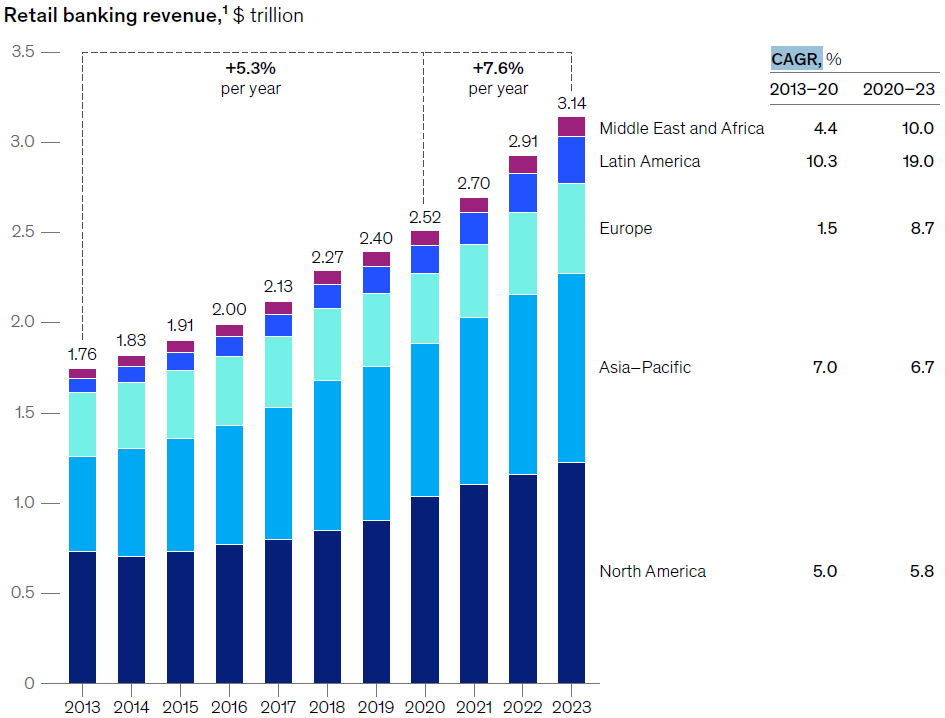
\includegraphics[]{Crowdfunding/figures/GlobalRetailLendingMarket_OnlyBank_ByArea.png}
    } %end of resizebox
%-----------------------------------------------
% Figure setting: caption and label
%-----------------------------------------------
\end{figure}
%-----------------------------------------------
\vspace{-3mm}








	
\end{frame} 
%----------------------------------------------------  




%------------------------------------------------

\begin{frame}
\frametitle{Retail Lending Sector Facts}



{\footnotesize Unlike regulated banks, public data is not reliable for Non-bank financial institutions, crowdfunding \& P2P platforms, and FinTech lenders!} 


\medskip 

However, Philipp Schnabl (NYU) and Manasa Gopal (Georgia Tech) study Uniform Commercial Code (``\textbf{UCC}'') filings of securitized, non-real-estate U.S. business loans made by non-banks (``fintechs'')

{\small 
\begin{itemize}
    \item Creditors have the right to file a record with the UCC registry specifying a loan and the underlying collateral, which is referred to as a ``UCC filing". 
    \item A UCC filing records the security interest in the underlying asset, analogous to mortgages for real estate, and determines the priority order of creditors in bankruptcy.
    \item If the borrower pledges a piece of collateral to multiple lenders, the lender with the earliest filing date has priority over other lenders.
\end{itemize}
 }


	
\end{frame} 
%----------------------------------------------------  




%------------------------------------------------

\begin{frame}
\frametitle{Retail Lending Sector Pain Points}




\vspace{-5mm}
%-----------------------------------------------
\begin{figure}[H]
    \resizebox{4.6in}{2in}{%
    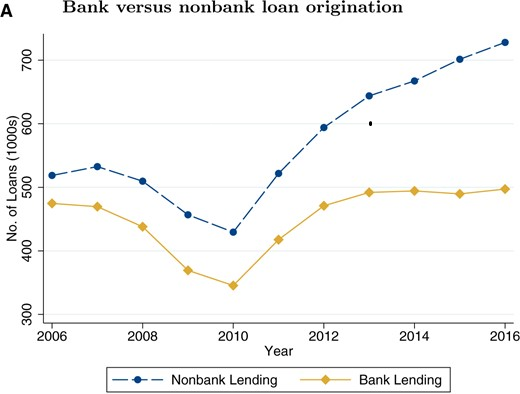
\includegraphics[]{Crowdfunding/figures/GrowthOfNonbankLending_Post2008.png}
    } %end of resizebox
%-----------------------------------------------
% Figure setting: caption and label
%-----------------------------------------------
\end{figure}
%-----------------------------------------------
\vspace{-3mm}
{\footnotesize Note: nonbank lending here includes all lending that are not by bank. }

\smallskip 
\vspace{1mm}


Schnabl \& Gopal (2022) find that heavier regulatory cost on banks post-2008 is one explanation for the relatively faster growth of nonbank lending.

\end{frame} 
%----------------------------------------------------  





%------------------------------------------------

\begin{frame}
\frametitle{Retail Lending Sector Pain Points}


What are the pain points that crowdfunding companies try to solve? \\
\smallskip 
\textbf{For Fundraisers (Borrowers / Issuers):}
\begin{itemize}
    \item \textbf{Access to Capital} -- bypasses traditional gatekeepers (banks and VCs are inaccessible for early-stage or non-traditional ventures.)
    \item \textbf{Speed \& Simplicity} -- fast online application and launch than with traditional banks and VCs.
    \item \textbf{Market Validation} -- test product/idea demand from early supporters, not possible with banks or VCs.
    \item \textbf{Lower Fundraising Costs} -- fewer legal/admin burdens than banks.
    \item \textbf{Audience Engagement} -- build community and future customers, not possible with banks or VCs.
\end{itemize}



	
\end{frame} 
%----------------------------------------------------  




%------------------------------------------------

\begin{frame}
\frametitle{Retail Lending Sector Pain Points}


What are the pain points that crowdfunding companies try to solve? \\
\smallskip 
\textbf{For Funders (Investors / Backers):}
\begin{itemize}
    \item \textbf{Access to New Opportunities} -- invest in startups, real estate, or social ventures that were traditionally reserved for accredited investors or institutions.
    \item \textbf{Diversification} -- small minimums across many projects
    \item \textbf{Emotional/Social Return of Investment} -- support causes or innovations they believe in
\end{itemize}


	
\end{frame} 
%----------------------------------------------------  




%---------------------------------------------------- 
%---------------------------------------------------- 
\section{Crowdfunding}
%---------------------------------------------------- 
%---------------------------------------------------- 




%---------------------------------------------------- 
\subsection{Crowdfunding Basics}
%---------------------------------------------------- 




%------------------------------------------------

\begin{frame}
\frametitle{Crowdfunding Basics}

\begin{itemize}
    \item Crowdfunding platforms allow individuals, businesses, and social causes to raise capital directly from the crowd in the form of debt, equity, donations, or rewards
    \begin{itemize}
        \item Also called alternative finance
        \item Debt crowdfunding platforms are Commonly called peer-to-peer (P2P) lenders or marketplace lenders
    \end{itemize}

    \medskip 

    \item These fintechs started between 2005 to 2009
    \begin{itemize}
        \item Zopa (UK), launched in 2005, was the pioneer among online portals
        \item OnDeck and Prosper launched in 2006; 
        \item CreditKarma and LendingClub in 2007; 
        \item Indiegogo and GoFundMe in 2008
        \item Funding Circle, Kabbage, and Kickstarter in 2009
    \end{itemize}

    \medskip 
    
    \item Described as the ``most disruptive way to raise money''
\end{itemize}


\end{frame} 
%----------------------------------------------------  






%------------------------------------------------

\begin{frame}
\frametitle{Crowdfunding Basics}

\begin{itemize}
    \item Technology made crowdfunding possible
    \begin{itemize}
        \item Fintechs leveraged the internet, mobile phones, software, APIs, cloud computing, and social media
    \end{itemize}
    \medskip 
    \item Platform growth
    \begin{itemize}
        \item In 2022, Crunchbase reported 1,500 active crowdfunding platforms headquartered in the USA
        \item An additional 200 platforms had closed
    \end{itemize}
    \medskip 
    \item Evolution of funding sources
    \begin{itemize}
        \item Originally crowdfunding was P2P, connecting individuals with retail investors ("the crowd")
        \item Now, most funding comes from institutional investors:
        \begin{itemize}
            \item Hedge funds, pension funds, insurance companies, banks, and professional investors
        \end{itemize}
        \item To reflect this broader capital source, the term \textbf{marketplace lending} is used
    \end{itemize}
\end{itemize}


\end{frame} 
%----------------------------------------------------  





%------------------------------------------------

\begin{frame}
\frametitle{Crowdfunding Basics}

\vspace{-2mm}
Business Models
\begin{itemize}
    \item Many crowdfunding platforms are multi-sided markets with users on various sides
    \item Network effects are crucial: a higher number of users increases the value to:
    \begin{itemize}
        \item The platform operator; The entity raising capital; The crowd(funders)
    \end{itemize}
\end{itemize}


\vspace{-3mm}
%-----------------------------------------------
\begin{figure}[H]
    \resizebox{4in}{1.8in}{%
    
\includegraphics[]{Crowdfunding/figures/NetworkEffect.png}
    } %end of resizebox
%-----------------------------------------------
% Figure setting: caption and label
%-----------------------------------------------
\end{figure}
%-----------------------------------------------
\vspace{-3mm}




\end{frame} 
%----------------------------------------------------  










%------------------------------------------------

\begin{frame}
\frametitle{Crowdfunding Basics}

As crowdfunding finance has matured, \textcolor{red}{the hope} that online portals would disrupt banks and transform capital raising \textcolor{red}{has faded}.
\medskip 
\begin{itemize}
    \item Challenges faced by online portals
    \begin{itemize}
        \item Struggled to monetize users and cover the high customer acquisition costs: estimated at \$500 to \$1,000 per customer
        \item Disclosures of the largest, publicly listed online portals show years of losses with share prices falling steadily.
    \end{itemize}
    \medskip 
    \item Many platforms have pivoted from their original vision
    \begin{itemize}
        \item Closed to retail investors: Zopa, Prosper
        \item Became digital banks: LendingClub, SoFi
        \item Acquired by incumbents: Kabbage, OnDeck
        \item Many went bankrupt and disappeared
    \end{itemize}
\end{itemize}



\end{frame} 
%----------------------------------------------------  






%------------------------------------------------

\begin{frame}
\frametitle{Crowdfunding Basics}


Regarding the five dimensions of financial intermediation, Crowdfunding portals have succeeded in some areas but failed in others:

\begin{itemize}
    \item Reduced information asymmetry between savers and borrowers/investors by increasing disclosure


    \item Mixed on transaction costs; lowered the cost and increased the speed to post a campaign, but charge high origination fees and high interest rates.


    \item Do not solve the liquidity problem; little ability to resell securities purchased on a crowdfunding platform.


    \item Do not provide risk sharing; investors bear the risks of default. Crowdfunding portal has no skin-in-the-game. 


    \item Have not built trust with episodes of fraud, misrepresentation, and principal-agent problems found in the traditional financial system.

\end{itemize}




\end{frame} 
%----------------------------------------------------  




%------------------------------------------------

\begin{frame}
\frametitle{Crowdfunding Basics}

\vspace{-2mm }
Two types of crowdfunding:
\begin{itemize}
    \item \textbf{Investment}: debt or equity investors for return
    \item \textbf{Non-investment}: donate money to charities \& people
\end{itemize}


\vspace{-5mm}
%-----------------------------------------------
\begin{figure}[H]
    \resizebox{5.6in}{2.2in}{%
    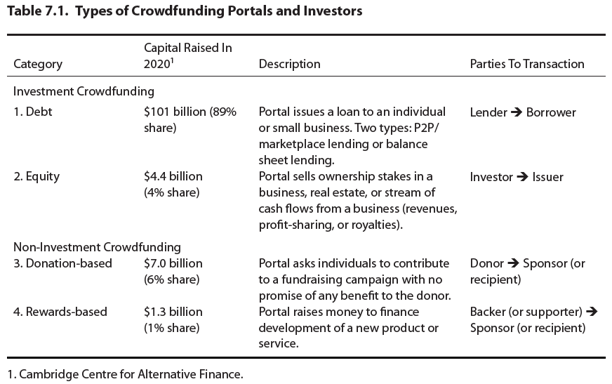
\includegraphics[]{Crowdfunding/figures/TypeOfCroudfunding.png}
    } %end of resizebox
%-----------------------------------------------
% Figure setting: caption and label
%-----------------------------------------------
\end{figure}
%-----------------------------------------------
\vspace{-3mm}




\end{frame} 
%----------------------------------------------------  



\section{Housekeeping}

\begin{frame}{Final Projects}

\begin{itemize}
    \item Presentation Videos or Slideshows are limited to \textbf{Two Minutes} per participant -- \textbf{be succinct!!} 
    \item Live Q\&A will follow each presentation (I am the questioner) \pause 
    \item If you are doing a \textbf{Min-Thesis}: 
    \begin{itemize}
        \item The title slide should be the thesis statement, a grammatically-complete sentence. 
        \item The first slide should clearly define your data source(s) and variables 
        \item The last slide should clearly state what the visualizations \textbf{would have looked like, were your thesis statement false}. 
    \end{itemize} \pause 
    \item If you are doing a \textbf{Smart Contract}: 
    \begin{itemize}
        \item I recommend making a demo video rather than demonstrating live 
        \item Please \textbf{include audio} so we can understand what your contract is doing 
        \item \textbf{Showmanship} is valuable! 1/10 of the grade will be based on showmanship. \textbf{Marketing is part of your job}. 
    \end{itemize}
\end{itemize}
    
\end{frame}


\section{In the News}

\begin{frame}{Trump CFPB Dismisses Moneygram Complaint}

\begin{center}
    
\includegraphics[height = .9\textheight]{moneygram_headline.png}
\end{center}
    
\end{frame}

\begin{frame}{Moneygram Business Model}

\begin{center}
    
\includegraphics[width = \textwidth]{moneygram_description.png}
\end{center}
    
\end{frame}

\begin{frame}{Moneygram Complaint}

\begin{center}
    
\includegraphics[width = \textwidth]{moneygram_complaint.png}
\end{center}
    
\end{frame}

\begin{frame}{Other Regulations Binding Moneygram}

\begin{center}
    
\includegraphics[width = \textwidth]{moneygram_AML.png}
\end{center}
    
\end{frame}


\section{Crowdfunding, Cont.}

%------------------------------------------------
%------------------------------------------------
\subsection{Types: Online Lending, Equity Crowdfunding, Donations \& Rewards}
%------------------------------------------------
%------------------------------------------------


%------------------------------------------------

\begin{frame}
\frametitle{Online Lending}

Correia (UGA), Han, and Wang (UIUC) study online loans made through online lenders like \href{https://greendayonline.com/online-loan-application/}{Green Day Online} and compare them to traditional ``storefront'' loans. 
 \vfill 
They find that, even looking at different loans made to \emph{the same borrower}, online loans have \textbf{higher interest rates} and \textbf{higher default rates}
 \vfill 
Not explained by differences in collateral, contract design, or credit score implications 
\vfill 
In addition to within-borrower effects, online lenders face \textbf{negative selection}: worse borrowers are more likely to seek loans online 

\end{frame} 
%----------------------------------------------------  

\begin{frame}{Online vs. Storefront Loans}

\begin{center}
    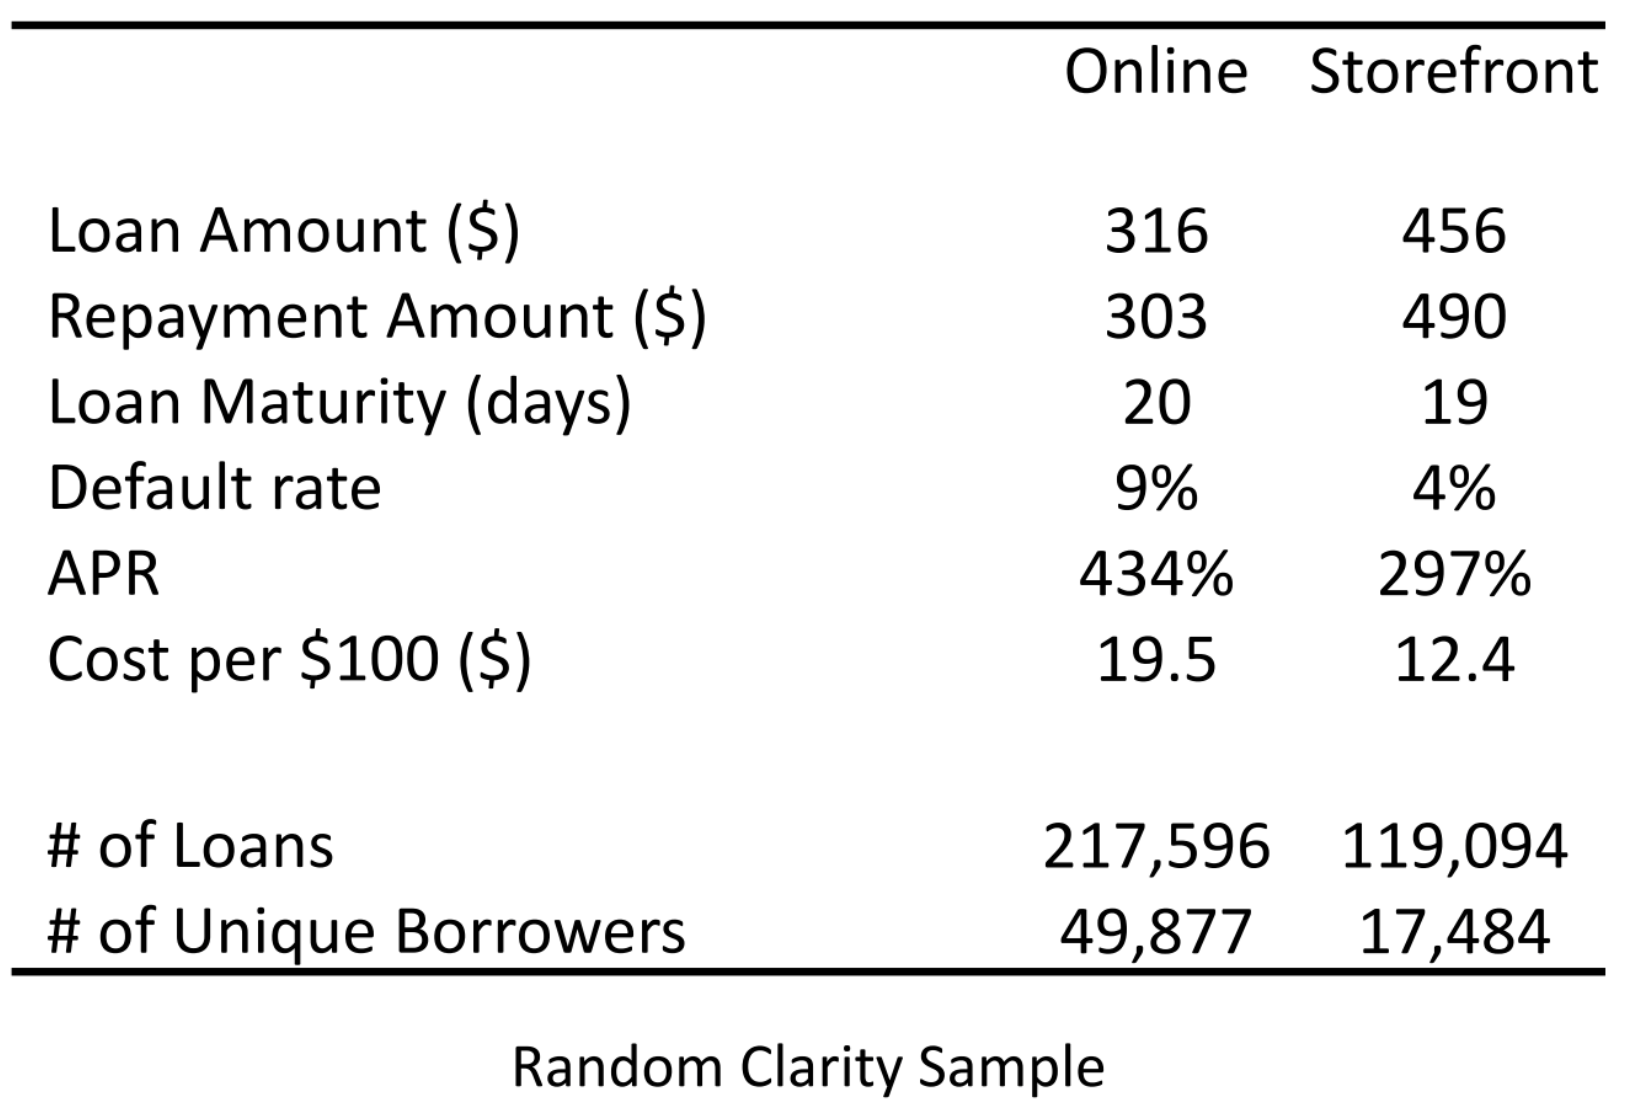
\includegraphics[height = .8\textheight]{Crowdfunding/online_loan_table.png}
\end{center}
    
\end{frame}


%------------------------------------------------

\begin{frame}
\frametitle{Individual vs Business Borrowers}



    \begin{itemize}
        \item Individuals borrow up to \$50,000 and small businesses up to \$500,000 for terms up to 5 years.
        \begin{itemize}
            \item US study (2012-17): avg online borrower is 49 year old with below average credit score borrowing \$8,500 for 3.25 years.
        \end{itemize}
        \item Small businesses have increasingly turned to online lenders to access capital, raising \$43 billion or 43\% of online lending globally in 2020.
    \end{itemize}



\end{frame} 
%----------------------------------------------------  



%------------------------------------------------

\begin{frame}
\frametitle{Comparison of Marketplace Lenders}


%-----------------------------------------------
\begin{figure}[H]
    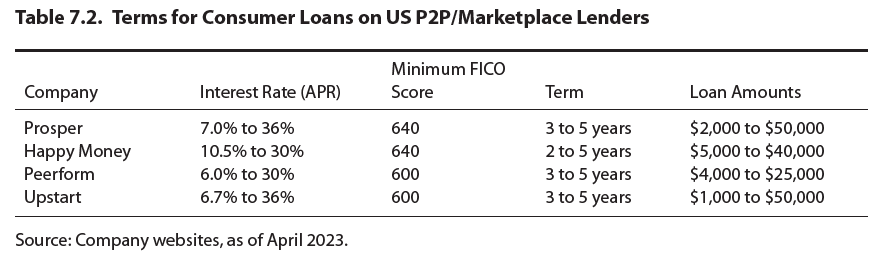
\includegraphics[width = \textwidth]{Crowdfunding/figures/MarketplaceLenders_InterestRate_Fees.png}
%-----------------------------------------------
% Figure setting: caption and label
%-----------------------------------------------
\end{figure}
%-----------------------------------------------



\end{frame} 
%----------------------------------------------------  





%------------------------------------------------

\begin{frame}
\frametitle{Crowdfunding Online Debt Lending}


Institutional investors have leveraged technology to automate the investment process. 
\begin{itemize}
    \item Connect to portal using API, screen and analyze postings in real-time using proprietary computer algorithms (or robots) that make decision to invest or not.
    \item A study of LendingClub found that robot investors outperformed less sophisticated investors. 
\end{itemize}

\medskip 

Does marketplace lending increase financial inclusion?
\begin{itemize}
    \item Some studies find that AI can identify “invisible prime” borrowers who are turned down by traditional lenders due to low FICO scores but are more creditworthy. 
    \item Overall, evidence is mixed, with no clear consensus in the literature on whether AI can meaningfully outperform traditional credit scores. 
\end{itemize}


\end{frame} 
%----------------------------------------------------  




%------------------------------------------------

\begin{frame}
\frametitle{Case Study: Lendified – Using Artificial Intelligence}


Lendified is fully automated balance sheet lender for small and medium enterprises (SMEs)
\begin{itemize}
    \item Founded in Toronto 2015 by two ex-bankers
    \item Offers loans up to \$150,000 with terms up to 24 months
\end{itemize}

\medskip 


Businesses apply online (under 10 minutes), get an instant decision, and receive funding in 48 hours
\begin{itemize}
    \item Lendified’s software, Judi.ai, connects via API to the applicant’s bank account and generates a cash flow forecast. This forecast is analyzed by a proprietary credit engine to evaluate the ability to finance the loan.
    \item Loan may be collateralized by inventory or accounts receivable to reduce the risk and the cost of borrowing.
    \item Cut loan adjudication costs by 90\%, make decision in minutes, not weeks.
\end{itemize}


\end{frame} 
%----------------------------------------------------  



%----------------------------------------------------  
%----------------------------------------------------  
%----------------------------------------------------  
%----------------------------------------------------  





%------------------------------------------------

\begin{frame}
\frametitle{Crowdfunding Online Equity Issuance}


Regulation of equity crowdfunding: Most start-ups fail so regulators limit how much retail investors may invest in any campaign
\begin{itemize}
    \item SEC's 2024 ``Regulation Crowdfunding'' sets limit on investment at greater of \$2,200 or 5\% of annual income up to \$150,000 (or 10\% of annual income above \$150,000). \href{https://www.sec.gov/education/smallbusiness/exemptofferings/regcrowdfunding}{SEC Regulation on Equity Crowdfunding}
    \item Canada sets cap at CA\$2,500 per deal, or CA\$10,000 if a registered dealer has supplied advice
    \item Other platforms restricted to accredited (high net–worth) investors, such as AngelList
\end{itemize}


\end{frame} 
%----------------------------------------------------  








%------------------------------------------------

%----------------------------------------------------  
%----------------------------------------------------  
%----------------------------------------------------  
%----------------------------------------------------  



%------------------------------------------------

\begin{frame}
\frametitle{Donations and Rewards Crowdfunding}


\begin{itemize}
    \item Donation-based crowdfunding ask individuals to contribute to a fundraising campaign with no promise of any benefit to the donor
    \begin{itemize}
        \item Artistic projects, civic projects, charities, medical expenses, or disaster relief.
        \smallskip 
        \item GoFundMe is the world's largest with \$5 billion+ raised.
    \end{itemize}
    \medskip 
    \item Rewards-based crowdfunding raises money to finance the development of a new product or service. 
    \begin{itemize}
        \item Entrepreneur pre-sells a future product to backers (or supporters) who are promised a reward when the project is completed.
        \smallskip
        \item Kickstarter and Indiegogo are biggest in USA.
    \end{itemize}
\end{itemize}



\end{frame} 
%----------------------------------------------------  





%------------------------------------------------

\begin{frame}
\frametitle{Case: Kickstarter Brings Creative Projects to Life}

Support Art, Comics, Crafts, Dance, Design, Fashion, Film \& Video, Food, Games, Journalism, Music, Photography, Publishing, Technology, and Theater.
\begin{itemize}
    \item Since launch in 2009, 23 million people pledged \$7.75 billion of which 250,000+ projects funded (41\% success)
    \item Most successful projects raise less than \$10,000, but close to 800 have raised \$1 million+
    \begin{itemize}
        \item Pebble Time smartwatch (\$20 million), Veronica Mars movie project (\$6 million), Reading Rainbow project (\$5 million).
    \end{itemize}
    \item Creator sets goal and raises funding up to 60 days.
    \item Set up a project page with video and description that explains story behind creative project. Outline the rewards backers will receive when completed.
    \item Monetization: platform (underwriting) fee of 5\% of total funds raised, plus payment processing fee of 3\% + \$0.20 per pledge.
    \item \url{https://www.kickstarter.com/}
\end{itemize}



\end{frame} 
%----------------------------------------------------  



%------------------------------------------------

\begin{frame}
\frametitle{Crowdfunding is more successful in Equity, Donation, and Rewards}



\vspace{-2mm}
%-----------------------------------------------
\begin{figure}[H]
    \resizebox{5.6in}{2.6in}{%
    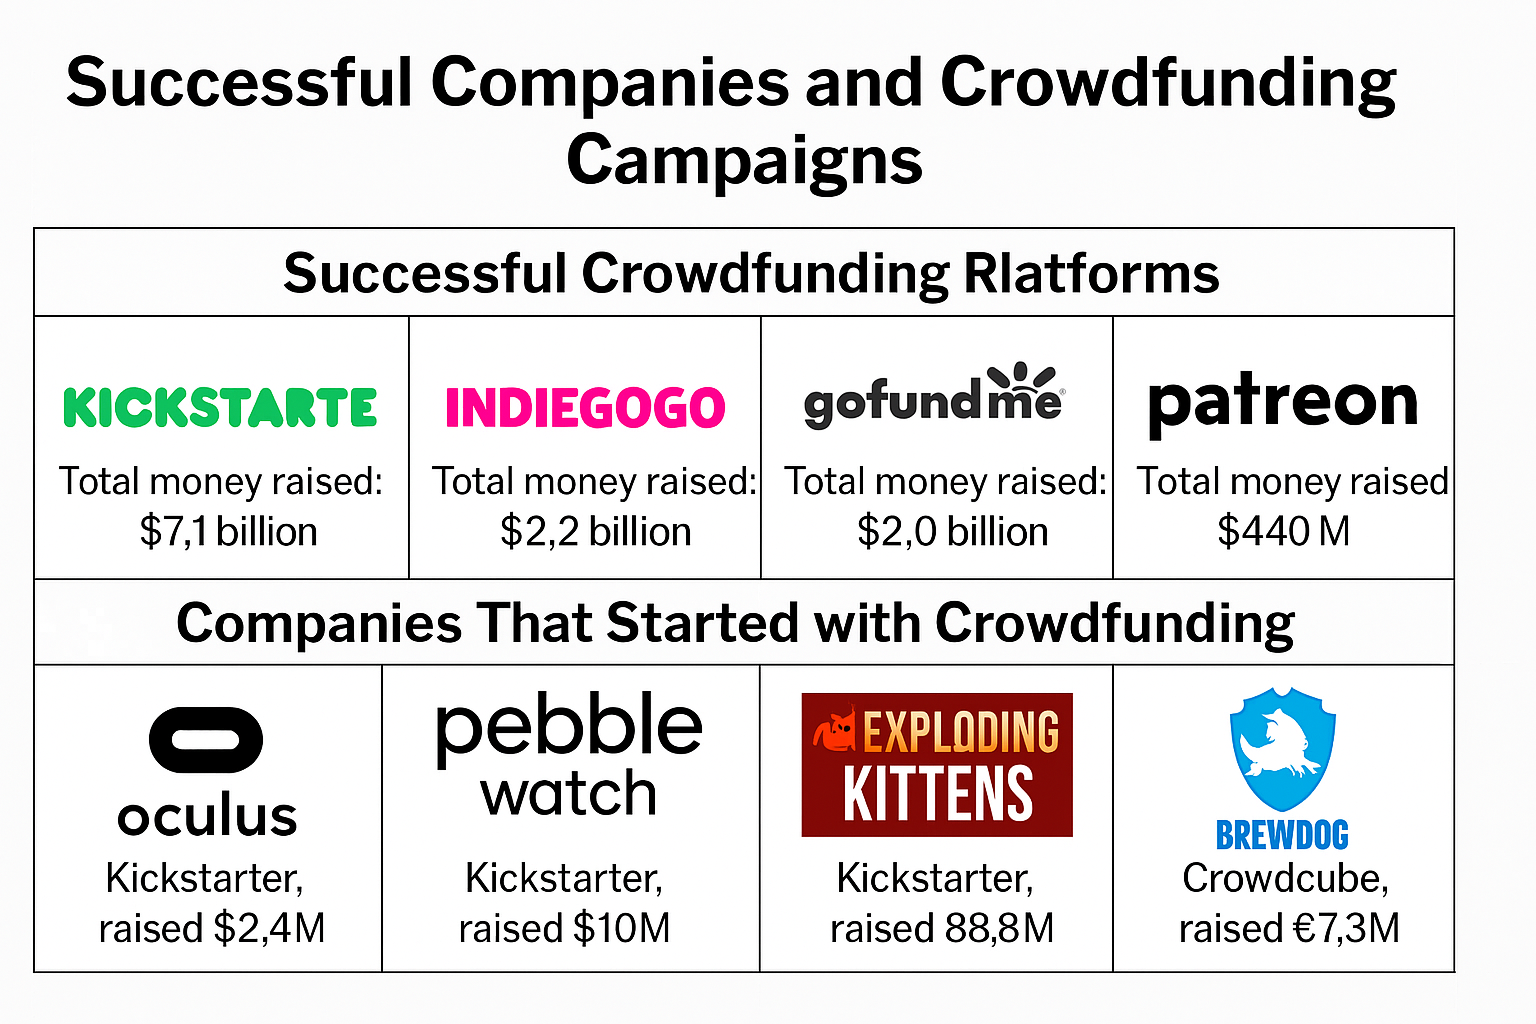
\includegraphics[]{Crowdfunding/figures/SuccessfulCrowdfundingPlatforms_Equity,Donation,Rewards.png}
    } %end of resizebox
%-----------------------------------------------
% Figure setting: caption and label
%-----------------------------------------------
\end{figure}
%-----------------------------------------------
\vspace{-2mm}





\end{frame} 
%----------------------------------------------------  




%----------------------------------------------------  
%----------------------------------------------------  

\subsection{The Rise and Fall of Crowdfunding Globally}

%----------------------------------------------------  
%---------------------------------------------------- 




%------------------------------------------------

\begin{frame}
\frametitle{The Rise and Fall of Crowdfunding Globally}


Alternative finance grew rapidly over 15 years, reaching US\$419 billion in 2017, with China reaching \textbf{86\% of the global market!} 

\medskip

\begin{itemize}
    \item Widespread fraud, bankruptcies and a regulatory crackdown saw of hundreds of Chinese portals close. Millions of investors lost their life savings.
    \medskip 
    
    \item Fraud case: Ezubao
    \begin{itemize}
        \item founded 2014, became one of China’s largest P2P platforms, raising \$8 billion within 2 years.
        \smallskip 
        \item In early 2016, news outlets reported that 20 people associated with the platform had been arrested for fraud. 
        \smallskip 
        \item Chinese retail investors staged protests in front of police stations, publicly blaming the platform operators and lax regulators for their losses.
    \end{itemize}
\end{itemize}

\end{frame} 
%----------------------------------------------------  




%------------------------------------------------

\begin{frame}
\frametitle{The Rise and Fall of Crowdfunding Globally}

\vspace{-2mm}
By 2020, \$114 billion was raised globally: USA 65\%, Europe 20\%, and China 1\%. 

\begin{itemize}
    \item Alternative finance has raised close to \$1.5 trillion over 2013-2020.
    \item Alternative finance was summarily banned entirely in China. 
    \item Ex-China growth continues. 
\end{itemize}

\vspace{-5mm}
%-----------------------------------------------
\begin{figure}[H]
    \resizebox{5.6in}{1.8in}{%
    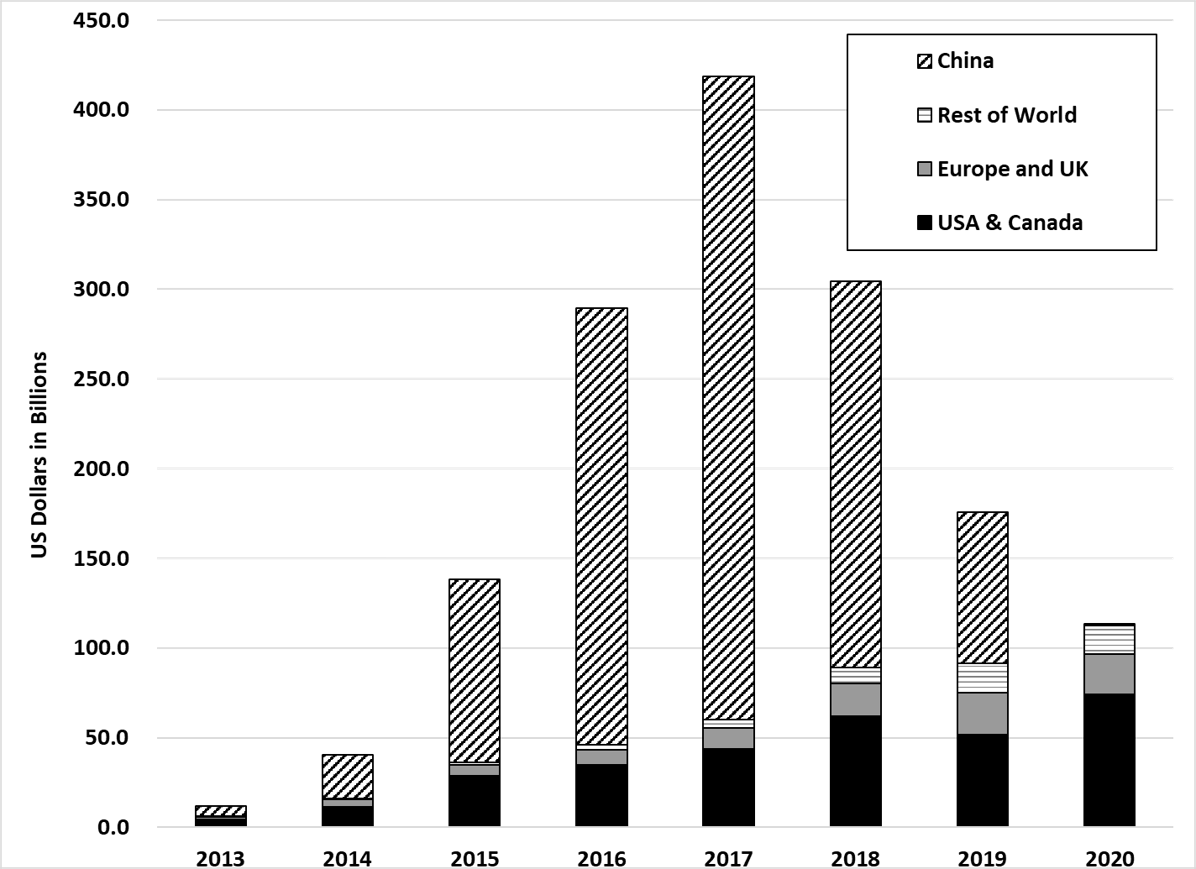
\includegraphics[]{Crowdfunding/figures/Rise&Fall_GlobalCroudfunding.png}
    } %end of resizebox
%-----------------------------------------------
% Figure setting: caption and label
%-----------------------------------------------
\end{figure}
%-----------------------------------------------
\vspace{-4mm}




\end{frame} 
%----------------------------------------------------  



%------------------------------------------------

\begin{frame}
\frametitle{The Rise and Fall of Crowdfunding Globally}

\vspace{-2mm}
Alternative Finance Market Size and Growth
\begin{itemize}
    \item In 2020, debt crowdfunding was 89\% of funding raised, equity 4\%, and non-investment (donation, rewards) 7\%.
\end{itemize}


\vspace{-5mm}
%-----------------------------------------------
\begin{figure}[H]
    \resizebox{5.6in}{2.2in}{%
    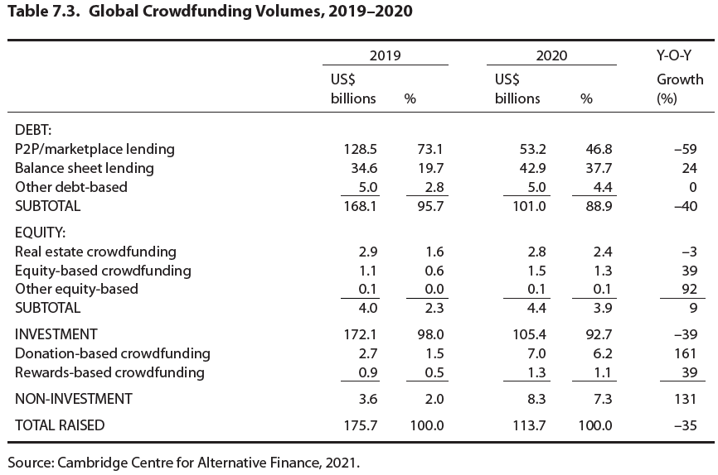
\includegraphics[]{Crowdfunding/figures/GlobalCroudfunding_Type_2019&2020.png}
    } %end of resizebox
%-----------------------------------------------
% Figure setting: caption and label
%-----------------------------------------------
\end{figure}
%-----------------------------------------------
\vspace{-4mm}



\end{frame} 
%----------------------------------------------------  



%------------------------------------------------



%------------------------------------------------


%------------------------------------------------

\begin{frame}
\frametitle{Regulations and Logistics}

Regulation is a high barrier to entry
\begin{itemize}
        \item U.S. crowdfunding platforms are covered by federal and state licensing requirements, consumer protection laws, securities laws, anti-money laundering laws, and national securities association (FINRA) rules.
        \item They must register with the U.S. Securities and Exchange Commission (SEC), become a FINRA member, and meet ongoing reporting and disclosure requirements.
    \end{itemize}

\medskip 

In 2016, the Office of the Comptroller of the Currency (OCC) announced plans to issue a special fintech charter that would allow online portals to be supervised federally and not by states.
\begin{itemize}
    \item Square \textcolor{red}{applied in 2017} and \textcolor{red}{received its charter in 2020}.
    \item SoFi \textcolor{red}{applied in 2017} and \textcolor{red}{received its charter in 2022}.
    \item Many fintechs have not applied, preferring to use banking-as-a-service 
\end{itemize}



\end{frame} 
%----------------------------------------------------  

%---------------------------------------------------- 
%---------------------------------------------------- 
\subsection{Business Model}
%---------------------------------------------------- 
%---------------------------------------------------- 



%------------------------------------------------

\begin{frame}
\frametitle{How Crowdfunding Portals Make Money}


They charge fees to users on various sides of their multi-sided platforms: (1) Issuers or borrowers on one side; (2) Investors or lenders on the other
 

\medskip 


\begin{itemize}
    \item Sign-up fee: may charge a listing fee regardless of success or failure of campaign
    \item Subscription fee: or charge a monthly or annual fee that allows issuers to run campaigns over a fixed period
    \item Underwriting fee: 1\% to 5\% of any capital raised
    \item Carry percentage / warrants: platform may invest in the campaign and share upside if successful
    \item Payment processing fee: 3\% on payments plus an amount per pledge paid (similar to a credit card issuer)
    \item Management fee: a percentage of assets under management (AUM)
\end{itemize}



\end{frame} 
%----------------------------------------------------  





%------------------------------------------------

\begin{frame}
\frametitle{How Crowdfunding Portals Make Money}


Online lending portals charge fees to both the borrower and the lender:
\begin{itemize}
    \item Loan interest rate: 6\% to 30\% APR, or more
    \item Origination fee: 3.0\% to 6.5\% of amount raised
    \item Late or missed payment fee: specified in the loan contract (called an indenture);
    \begin{itemize}
        \item Example: overdue payment fee equal to 15\% of missing loan payments
    \end{itemize}
    \item Servicing fee: 1\% to 3\% of each payment
    \item Marketing (or Transaction) fee: charge a bank, a hedge fund, or a high net–worth individual a fee to cover the expense of acquiring customers. LendingClub charges banks 1\% to 6\% of the face amount of the loan.
\end{itemize}



\end{frame} 
%----------------------------------------------------  



%------------------------------------------------

\begin{frame}
\frametitle{How Crowdfunding Portals Make Money}


Crowdfunding portals have same expenses as a traditional financial intermediary:
\begin{itemize}
    \item Sales and marketing expenses (cost of customer acquisition)
    \item Technology costs
    \item Research and development
    \item Salaries, benefits, and employee compensation
    \item General and administrative expenses (e.g., overhead)
    \item Distribution, processing, and servicing costs
    \item Corporate taxes
    \item Funding costs for balance sheet lenders
    \item Write-downs on non-performing loans for balance sheet lenders
\end{itemize}



\end{frame} 
%----------------------------------------------------  





%---------------------------------------------------- 
%---------------------------------------------------- 
\subsection{Crowdfunding Research Findings}
%---------------------------------------------------- 
%---------------------------------------------------- 


%------------------------------------------------

\begin{frame}
\frametitle{Crowdfunding Research Findings: Mixed Evidence}


Competition and Financial Inclusion
\begin{itemize}
    \item Entered markets with fewer bank branches, lower incomes, more minority households, underbanked rural communities, industries with fewer banking relationships,
    \item Entered markets where complaints about bank misconduct are higher, and where banks have pulled back during past economic downturns (including 2008 global financial crisis).
\end{itemize}

\medskip 

Other studies disagree, saying they target borrowers with higher credit scores and education
\begin{itemize}
    \item Online lenders do not target risky or marginal borrowers who have low access to finance, but instead provide credit to borrowers who already have access via banks.
    \item Fintech mortgage lenders process mortgage applications 20\% faster than other lenders but charge a premium interest rate and serve more educated and older borrowers with good access to finance.
\end{itemize}



\end{frame} 
%----------------------------------------------------  




%------------------------------------------------

\begin{frame}
\frametitle{Crowdfunding Research Findings: Mixed Evidence}


Discrimination and Bias in Alternative Finance
\begin{itemize}
    \item Female entrepreneurs represented only 35\% of Kickstarter campaigns but had higher funding success.
    \item Experienced male and female investors show no gender bias when investing in projects. But inexperienced female investors favored female founders.
    \item African American men are significantly less likely than similar white founders to receive equity crowdfunding.
    \item Latinx (Latin American origin) and African American borrowers were charged significantly higher interest rates on online mortgages.
    \item Algorithmic decision-making tools such as machine learning may incorporate bias. When trained on data that itself incorporates human biases based on gender, race, income levels, and other factors.
\end{itemize}



\end{frame} 
%----------------------------------------------------  



%----------------------------------------------------  
%----------------------------------------------------  
\subsection{Case: LendingClub}
%----------------------------------------------------  
%----------------------------------------------------  



%------------------------------------------------

\begin{frame}
\frametitle{Case: LendingClub's Marketplace Lending Platform}



\vspace{-2mm}
%-----------------------------------------------
\begin{figure}[H]
    \resizebox{4in}{0.8in}{%
    
\includegraphics[]{Crowdfunding/figures/LendingClub_Logo.jpeg}
    } %end of resizebox
%-----------------------------------------------
% Figure setting: caption and label
%-----------------------------------------------
\end{figure}
%-----------------------------------------------
\vspace{-2mm}


\vspace{-2mm}
LendingClub is a U.S.-based financial technology company known for launching one of the first major peer-to-peer (P2P) lending platforms in the world. 
\medskip 
\begin{itemize}
    \item Founded in 2006, it began as a marketplace where individual borrowers could access personal loans funded by individual or institutional investors.
    \medskip 
    \item 2007: Becomes the first P2P lender to register its offerings with the SEC
    \medskip 
    \item 2014: Went public on the NYSE, raising \$870 million — one of the largest fintech IPOs
    \medskip 
    \item 2021: Acquired Radius Bank, becoming a fully chartered digital bank — a major pivot from marketplace lending to traditional banking
\end{itemize}


\end{frame} 
%----------------------------------------------------  




%------------------------------------------------

\begin{frame}
\frametitle{Case: LendingClub's Marketplace Lending Platform}


\footnotesize
\begin{columns}[T]
    % Left Column: Years 2007-2015
    \begin{column}{0.48\textwidth}
        \begin{tabular}{rlp{3.5cm}}
            \toprule
            \textbf{Year} & \textbf{Billion} & \textbf{Key Events} \\
            \midrule
            2007 & 0.002 & Launched as Facebook app \\
            2008 & 0.01 & Early P2P lending model \\
            2009 & 0.03 & Shift to direct lending \\
            2010 & 0.2 & Secures major funding \\
            2011 & 0.5 & Institutional investors join \\
            2012 & 1.0 & Expands loan categories \\
            2013 & 2.1 & Prepares for IPO \\
            2014 & 4.3 & Goes public (NYSE: LC) \\
            2015 & 8.4 & Record growth post-IPO \\
            \bottomrule
        \end{tabular}
    \end{column}

    % Right Column: Years 2016-2024
    \begin{column}{0.48\textwidth}
        \begin{tabular}{rlp{3.5cm}}
            \toprule
            \textbf{Year} & \textbf{Billion} & \textbf{Key Events} \\
            \midrule
            2016 & 8.8 & CEO resignation scandal \\
            2017 & 7.9 & Regulatory crackdown \\
            2018 & 10.9 & Acquires Radius Bank \\
            2019 & 12.2 & Peak origination volume \\
            2020 & 4.3 & COVID-19 shutdowns \\
            2021 & 10.4 & Rebound; digital banking push \\
            2022 & 13.1 & steady growth \\
            2023 & 7.4 & Rate hikes slow lending \\
            \bottomrule
        \end{tabular}
    \end{column}
\end{columns}




\end{frame} 
%----------------------------------------------------  







%------------------------------------------------

\begin{frame}
\frametitle{Case: LendingClub's Marketplace Lending Platform}

\vspace{-2mm}
LendingClub was listed on the NYSE in 2014 at \$15.00 per share
\begin{itemize}
    \item LC had originated \$6 billion in loans over 7-years but was still unprofitable.
    \item The stock price rose to \$25.74, then declined steadily.
\end{itemize}



\vspace{-2mm}
%-----------------------------------------------
\begin{figure}[H]
    \resizebox{5in}{2in}{%
    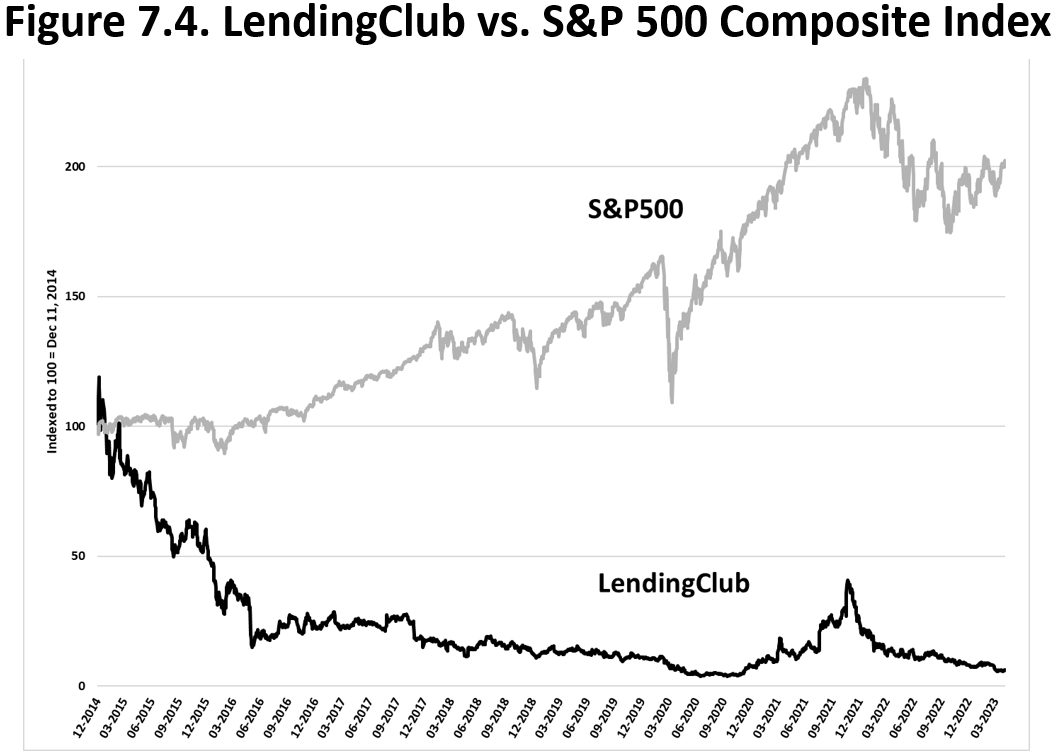
\includegraphics[]{Crowdfunding/figures/LendingClub_vs_S&P500.png}
    } %end of resizebox
%-----------------------------------------------
% Figure setting: caption and label
%-----------------------------------------------
\end{figure}
%-----------------------------------------------
\vspace{-2mm}



\end{frame} 
%----------------------------------------------------  




%----------------------------------------------------  
%----------------------------------------------------  
\subsection{Case: SoFi}
%----------------------------------------------------  
%----------------------------------------------------  


%------------------------------------------------

\begin{frame}
\frametitle{Case: SoFi’s Evolution from Online Lender to Full-Service Bank}

\vspace{-2mm}
Social Finance (SoFi) was founded as a P2P lender

\begin{itemize}
    \item Started in San Francisco in 2011 by four Stanford business school students who saw gap for alumni to fund MBA students at leading U.S. universities.
    \begin{itemize}
        \item By 2013, SoFi had funded \$200 million in loans to 2,500 undergraduate and graduate students at 100 eligible schools.
        \item SoFi moved away from this base, raising funding from  angels, VCs and banks. They securitized their loan book.
        \item They focused on building relationships with former borrowers (called members) through singles events, wine tastings, career counseling, and home-buying workshops.
    \end{itemize}
\end{itemize}

\medskip 

SoFi has grown to become a one-stop shop for financial services that allows members to borrow, save, spend, invest, and protect their money.
\begin{itemize}
    \item In mid-2021, SoFi went public in a SPAC-related IPO that valued the fintech at \$9 billion.
    \item SoFi was the largest non-bank unsecured consumer lender in the United States.
\end{itemize}



\end{frame} 
%----------------------------------------------------  




%------------------------------------------------

\begin{frame}
\frametitle{Case: SoFi’s Evolution from Online Lender to Full-Service Bank}

\vspace{-2mm}
Despite the success and media attention, SoFi has lost money in its last three fiscal years 

\begin{itemize}
    \item Operating expenses exceed revenues by a large margin
\end{itemize}


\vspace{-2mm}
%-----------------------------------------------
\begin{figure}[H]
    \resizebox{5in}{1.8in}{%
    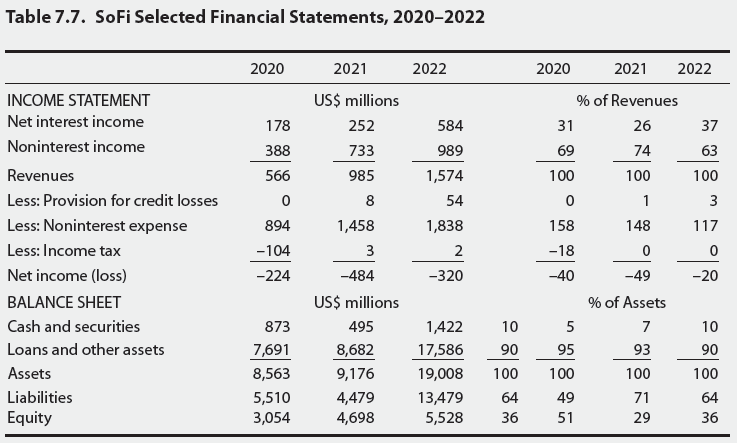
\includegraphics[]{Crowdfunding/figures/Sofi_FinancialStatement_2020To2022.png}
    } %end of resizebox
%-----------------------------------------------
% Figure setting: caption and label
%-----------------------------------------------
\end{figure}
%-----------------------------------------------
\vspace{-4mm}



\end{frame} 
%----------------------------------------------------  


%----------------------------------------------------  
%----------------------------------------------------  
\section{Conclusion}
%----------------------------------------------------  
%----------------------------------------------------  



%------------------------------------------------

\begin{frame}
\frametitle{Conclusion}


Crowdfunding provides a new business model for fundraising that directly matches borrowers and lenders online, outside of traditional finance.

\medskip 

Crowdfunding is more successful for equity, donations, and rewards for good products (like pepwatch) and art projects that are not served well by traditional finance. 

\medskip 

Crowdfunding continues to grow but very slowly recently. 

\medskip 

However, crowdfunding struggles to compete with traditional finance in customers that have already been served because crowdfunding does not offer a much better method: 
\begin{itemize}
    \item reducing (information asymmetry-induced) adverse selection problem
    \begin{itemize}
        \item Credit bureau data is somewhat mature. Alternative data does not provide comprehensive advantages. 
    \end{itemize}
    \item reducing (information asymmetry-induced) moral hazard problem
    \begin{itemize}
        \item Traditional finance institutions are still good at monitoring
    \end{itemize}
\end{itemize}




\end{frame} 
%----------------------------------------------------  




































































%----------------------------------------------------  
%----------------------------------------------------  
%----------------------------------------------------  
%----------------------------------------------------

\end{document}